\documentclass{article}
\usepackage[utf8]{inputenc}
\usepackage{graphicx}
\usepackage{url}
\usepackage{xcolor}
\usepackage{caption} 
\usepackage{hyperref}
\hypersetup{
    colorlinks=true,
    linkcolor=green,
    filecolor=magenta,      
    urlcolor=blue,
}


\newcommand*{\helvetica}{\fontfamily{phv}\selectfont}
\newcommand*{\helveticanarrow}{\fontfamily{phv}\fontseries{mc}\selectfont}
\newcommand*{\hvnb}{\fontfamily{phv}\fontseries{bc}\selectfont}


\DeclareCaptionFont{quack}{\helveticanarrow}
\captionsetup{font=quack, labelfont=bf}

\begin{document}
\helveticanarrow

\begin{figure}
\begin{center}
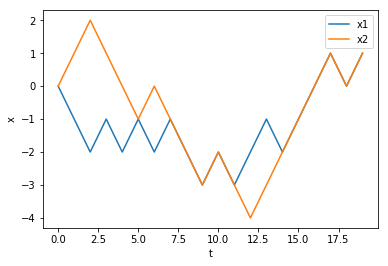
\includegraphics[width=0.9\textwidth]{./image.png}
\end{center}
\caption{Some random walks.  \href{https://mybinder.org/v2/gh/colm-connaughton/figure-test.git/master?filepath=figure.ipynb}{Click here to play with the code}. }
\end{figure}

\end{document}
